\begin{frame}[fragile]{Criação do DAG para a expressão \code{apl}{a + a × (b - c) + (b - c) × d}}

    \begin{tikzpicture}
        \node[opacity=0] at (0, 0) { y };
        \node[opacity=0] at (14, 7) { t };

        \node[anchor=west] at (0, 6.75) { \textbf{Chamadas de funções} };
    \end{tikzpicture}

\end{frame}

\begin{frame}[fragile]{Criação do DAG para a expressão \code{apl}{a + a × (b - c) + (b - c) × d}}

    \begin{tikzpicture}
        \node[opacity=0] at (0, 0) { y };
        \node[opacity=0] at (14, 7) { t };

        \node[anchor=west] at (0, 6.75) { \textbf{Chamadas de funções} };
        \node[anchor=west] at (0.5, 6.0) { $p_1 := \Call{criarFolha}{\textbf{id}, p_a}$ };
%        \node[anchor=west] at (0.5, 5.5) { $p_2 := \Call{criarFolha}{\textbf{id}, p_a}$ };
%        \node[anchor=west] at (0.5, 5.0) { $p_3 := \Call{criarFolha}{\textbf{id}, p_a}$ };
%        \node[anchor=west] at (0.5, 4.5) { $p_4 := \Call{criarFolha}{\textbf{id}, p_a}$ };
%        \node[anchor=west] at (0.5, 4.0) { $p_5 := \Call{criarFolha}{\textbf{id}, p_a}$ };
%        \node[anchor=west] at (0.5, 3.5) { $p_6 := \Call{criarFolha}{\textbf{id}, p_a}$ };
%        \node[anchor=west] at (0.5, 3.0) { $p_7 := \Call{criarFolha}{\textbf{id}, p_a}$ };
%        \node[anchor=west] at (0.5, 2.5) { $p_8 := \Call{criarFolha}{\textbf{id}, p_a}$ };
%        \node[anchor=west] at (0.5, 2.0) { $p_9 := \Call{criarFolha}{\textbf{id}, p_a}$ };
%        \node[anchor=west] at (0.5, 1.5) { $p_10 := \Call{criarFolha}{\textbf{id}, p_a}$ };
%        \node[anchor=west] at (0.5, 1.0) { $p_11 := \Call{criarFolha}{\textbf{id}, p_a}$ };
%        \node[anchor=west] at (0.5, 0.5) { $p_12 := \Call{criarFolha}{\textbf{id}, p_a}$ };
%        \node[anchor=west] at (0.5, 0.0) { $p_13 := \Call{criarFolha}{\textbf{id}, p_a}$ };

    \end{tikzpicture}

\end{frame}

\begin{frame}[fragile]{Criação do DAG para a expressão \code{apl}{a + a × (b - c) + (b - c) × d}}

    \begin{tikzpicture}
        \node[opacity=0] at (0, 0) { y };
        \node[opacity=0] at (14, 7) { t };

        \node[anchor=west] at (0, 6.75) { \textbf{Chamadas de funções} };
        \node[anchor=west] at (0.5, 6.0) { $p_1 := \Call{criarFolha}{\textbf{id}, p_a}$ };
%        \node[anchor=west] at (0.5, 5.5) { $p_2 := \Call{criarFolha}{\textbf{id}, p_a}$ };
%        \node[anchor=west] at (0.5, 5.0) { $p_3 := \Call{criarFolha}{\textbf{id}, p_a}$ };
%        \node[anchor=west] at (0.5, 4.5) { $p_4 := \Call{criarFolha}{\textbf{id}, p_a}$ };
%        \node[anchor=west] at (0.5, 4.0) { $p_5 := \Call{criarFolha}{\textbf{id}, p_a}$ };
%        \node[anchor=west] at (0.5, 3.5) { $p_6 := \Call{criarFolha}{\textbf{id}, p_a}$ };
%        \node[anchor=west] at (0.5, 3.0) { $p_7 := \Call{criarFolha}{\textbf{id}, p_a}$ };
%        \node[anchor=west] at (0.5, 2.5) { $p_8 := \Call{criarFolha}{\textbf{id}, p_a}$ };
%        \node[anchor=west] at (0.5, 2.0) { $p_9 := \Call{criarFolha}{\textbf{id}, p_a}$ };
%        \node[anchor=west] at (0.5, 1.5) { $p_10 := \Call{criarFolha}{\textbf{id}, p_a}$ };
%        \node[anchor=west] at (0.5, 1.0) { $p_11 := \Call{criarFolha}{\textbf{id}, p_a}$ };
%        \node[anchor=west] at (0.5, 0.5) { $p_12 := \Call{criarFolha}{\textbf{id}, p_a}$ };
%        \node[anchor=west] at (0.5, 0.0) { $p_13 := \Call{criarFolha}{\textbf{id}, p_a}$ };

        \node (A) at (8, 2) { \Large \code{apl}{a} };

    \end{tikzpicture}

\end{frame}

\begin{frame}[fragile]{Criação do DAG para a expressão \code{apl}{a + a × (b - c) + (b - c) × d}}

    \begin{tikzpicture}
        \node[opacity=0] at (0, 0) { y };
        \node[opacity=0] at (14, 7) { t };

        \node[anchor=west] at (0, 6.75) { \textbf{Chamadas de funções} };
        \node[anchor=west] at (0.5, 6.0) { $p_1 := \Call{criarFolha}{\textbf{id}, p_a}$ };
        \node[anchor=west] at (0.5, 5.5) { $p_2 := \Call{criarFolha}{\textbf{id}, p_a}$ };
%        \node[anchor=west] at (0.5, 5.0) { $p_3 := \Call{criarFolha}{\textbf{id}, p_a}$ };
%        \node[anchor=west] at (0.5, 4.5) { $p_4 := \Call{criarFolha}{\textbf{id}, p_a}$ };
%        \node[anchor=west] at (0.5, 4.0) { $p_5 := \Call{criarFolha}{\textbf{id}, p_a}$ };
%        \node[anchor=west] at (0.5, 3.5) { $p_6 := \Call{criarFolha}{\textbf{id}, p_a}$ };
%        \node[anchor=west] at (0.5, 3.0) { $p_7 := \Call{criarFolha}{\textbf{id}, p_a}$ };
%        \node[anchor=west] at (0.5, 2.5) { $p_8 := \Call{criarFolha}{\textbf{id}, p_a}$ };
%        \node[anchor=west] at (0.5, 2.0) { $p_9 := \Call{criarFolha}{\textbf{id}, p_a}$ };
%        \node[anchor=west] at (0.5, 1.5) { $p_10 := \Call{criarFolha}{\textbf{id}, p_a}$ };
%        \node[anchor=west] at (0.5, 1.0) { $p_11 := \Call{criarFolha}{\textbf{id}, p_a}$ };
%        \node[anchor=west] at (0.5, 0.5) { $p_12 := \Call{criarFolha}{\textbf{id}, p_a}$ };
%        \node[anchor=west] at (0.5, 0.0) { $p_13 := \Call{criarFolha}{\textbf{id}, p_a}$ };

        \node (A) at (8, 2) { \Large \code{apl}{a} };

    \end{tikzpicture}

\end{frame}

\begin{frame}[fragile]{Criação do DAG para a expressão \code{apl}{a + a × (b - c) + (b - c) × d}}

    \begin{tikzpicture}
        \node[opacity=0] at (0, 0) { y };
        \node[opacity=0] at (14, 7) { t };

        \node[anchor=west] at (0, 6.75) { \textbf{Chamadas de funções} };
        \node[anchor=west] at (0.5, 6.0) { $p_1 := \Call{criarFolha}{\textbf{id}, p_a}$ };
        \node[anchor=west] at (0.5, 5.5) { $p_2 := \Call{criarFolha}{\textbf{id}, p_a}$ };
        \node[anchor=west] at (0.5, 5.0) { $p_3 := \Call{criarFolha}{\textbf{id}, p_b}$ };
%        \node[anchor=west] at (0.5, 4.5) { $p_4 := \Call{criarFolha}{\textbf{id}, p_a}$ };
%        \node[anchor=west] at (0.5, 4.0) { $p_5 := \Call{criarFolha}{\textbf{id}, p_a}$ };
%        \node[anchor=west] at (0.5, 3.5) { $p_6 := \Call{criarFolha}{\textbf{id}, p_a}$ };
%        \node[anchor=west] at (0.5, 3.0) { $p_7 := \Call{criarFolha}{\textbf{id}, p_a}$ };
%        \node[anchor=west] at (0.5, 2.5) { $p_8 := \Call{criarFolha}{\textbf{id}, p_a}$ };
%        \node[anchor=west] at (0.5, 2.0) { $p_9 := \Call{criarFolha}{\textbf{id}, p_a}$ };
%        \node[anchor=west] at (0.5, 1.5) { $p_10 := \Call{criarFolha}{\textbf{id}, p_a}$ };
%        \node[anchor=west] at (0.5, 1.0) { $p_11 := \Call{criarFolha}{\textbf{id}, p_a}$ };
%        \node[anchor=west] at (0.5, 0.5) { $p_12 := \Call{criarFolha}{\textbf{id}, p_a}$ };
%        \node[anchor=west] at (0.5, 0.0) { $p_13 := \Call{criarFolha}{\textbf{id}, p_a}$ };

        \node (A) at (8, 2) { \Large \code{apl}{a} };

    \end{tikzpicture}

\end{frame}

\begin{frame}[fragile]{Criação do DAG para a expressão \code{apl}{a + a × (b - c) + (b - c) × d}}

    \begin{tikzpicture}
        \node[opacity=0] at (0, 0) { y };
        \node[opacity=0] at (14, 7) { t };

        \node[anchor=west] at (0, 6.75) { \textbf{Chamadas de funções} };
        \node[anchor=west] at (0.5, 6.0) { $p_1 := \Call{criarFolha}{\textbf{id}, p_a}$ };
        \node[anchor=west] at (0.5, 5.5) { $p_2 := \Call{criarFolha}{\textbf{id}, p_a}$ };
        \node[anchor=west] at (0.5, 5.0) { $p_3 := \Call{criarFolha}{\textbf{id}, p_b}$ };
%        \node[anchor=west] at (0.5, 4.5) { $p_4 := \Call{criarFolha}{\textbf{id}, p_a}$ };
%        \node[anchor=west] at (0.5, 4.0) { $p_5 := \Call{criarFolha}{\textbf{id}, p_a}$ };
%        \node[anchor=west] at (0.5, 3.5) { $p_6 := \Call{criarFolha}{\textbf{id}, p_a}$ };
%        \node[anchor=west] at (0.5, 3.0) { $p_7 := \Call{criarFolha}{\textbf{id}, p_a}$ };
%        \node[anchor=west] at (0.5, 2.5) { $p_8 := \Call{criarFolha}{\textbf{id}, p_a}$ };
%        \node[anchor=west] at (0.5, 2.0) { $p_9 := \Call{criarFolha}{\textbf{id}, p_a}$ };
%        \node[anchor=west] at (0.5, 1.5) { $p_10 := \Call{criarFolha}{\textbf{id}, p_a}$ };
%        \node[anchor=west] at (0.5, 1.0) { $p_11 := \Call{criarFolha}{\textbf{id}, p_a}$ };
%        \node[anchor=west] at (0.5, 0.5) { $p_12 := \Call{criarFolha}{\textbf{id}, p_a}$ };
%        \node[anchor=west] at (0.5, 0.0) { $p_13 := \Call{criarFolha}{\textbf{id}, p_a}$ };

        \node (A) at (8, 2) { \Large \code{apl}{a} };
        \node (B) at (9, 0.5) { \Large \code{apl}{b} };

    \end{tikzpicture}

\end{frame}

\begin{frame}[fragile]{Criação do DAG para a expressão \code{apl}{a + a × (b - c) + (b - c) × d}}

    \begin{tikzpicture}
        \node[opacity=0] at (0, 0) { y };
        \node[opacity=0] at (14, 7) { t };

        \node[anchor=west] at (0, 6.75) { \textbf{Chamadas de funções} };
        \node[anchor=west] at (0.5, 6.0) { $p_1 := \Call{criarFolha}{\textbf{id}, p_a}$ };
        \node[anchor=west] at (0.5, 5.5) { $p_2 := \Call{criarFolha}{\textbf{id}, p_a}$ };
        \node[anchor=west] at (0.5, 5.0) { $p_3 := \Call{criarFolha}{\textbf{id}, p_b}$ };
        \node[anchor=west] at (0.5, 4.5) { $p_4 := \Call{criarFolha}{\textbf{id}, p_c}$ };
%        \node[anchor=west] at (0.5, 4.0) { $p_5 := \Call{criarFolha}{\textbf{id}, p_a}$ };
%        \node[anchor=west] at (0.5, 3.5) { $p_6 := \Call{criarFolha}{\textbf{id}, p_a}$ };
%        \node[anchor=west] at (0.5, 3.0) { $p_7 := \Call{criarFolha}{\textbf{id}, p_a}$ };
%        \node[anchor=west] at (0.5, 2.5) { $p_8 := \Call{criarFolha}{\textbf{id}, p_a}$ };
%        \node[anchor=west] at (0.5, 2.0) { $p_9 := \Call{criarFolha}{\textbf{id}, p_a}$ };
%        \node[anchor=west] at (0.5, 1.5) { $p_10 := \Call{criarFolha}{\textbf{id}, p_a}$ };
%        \node[anchor=west] at (0.5, 1.0) { $p_11 := \Call{criarFolha}{\textbf{id}, p_a}$ };
%        \node[anchor=west] at (0.5, 0.5) { $p_12 := \Call{criarFolha}{\textbf{id}, p_a}$ };
%        \node[anchor=west] at (0.5, 0.0) { $p_13 := \Call{criarFolha}{\textbf{id}, p_a}$ };

        \node (A) at (8, 2) { \Large \code{apl}{a} };
        \node (B) at (9, 0.5) { \Large \code{apl}{b} };

    \end{tikzpicture}

\end{frame}

\begin{frame}[fragile]{Criação do DAG para a expressão \code{apl}{a + a × (b - c) + (b - c) × d}}

    \begin{tikzpicture}
        \node[opacity=0] at (0, 0) { y };
        \node[opacity=0] at (14, 7) { t };

        \node[anchor=west] at (0, 6.75) { \textbf{Chamadas de funções} };
        \node[anchor=west] at (0.5, 6.0) { $p_1 := \Call{criarFolha}{\textbf{id}, p_a}$ };
        \node[anchor=west] at (0.5, 5.5) { $p_2 := \Call{criarFolha}{\textbf{id}, p_a}$ };
        \node[anchor=west] at (0.5, 5.0) { $p_3 := \Call{criarFolha}{\textbf{id}, p_b}$ };
        \node[anchor=west] at (0.5, 4.5) { $p_4 := \Call{criarFolha}{\textbf{id}, p_c}$ };
%        \node[anchor=west] at (0.5, 4.0) { $p_5 := \Call{criarFolha}{\textbf{id}, p_a}$ };
%        \node[anchor=west] at (0.5, 3.5) { $p_6 := \Call{criarFolha}{\textbf{id}, p_a}$ };
%        \node[anchor=west] at (0.5, 3.0) { $p_7 := \Call{criarFolha}{\textbf{id}, p_a}$ };
%        \node[anchor=west] at (0.5, 2.5) { $p_8 := \Call{criarFolha}{\textbf{id}, p_a}$ };
%        \node[anchor=west] at (0.5, 2.0) { $p_9 := \Call{criarFolha}{\textbf{id}, p_a}$ };
%        \node[anchor=west] at (0.5, 1.5) { $p_10 := \Call{criarFolha}{\textbf{id}, p_a}$ };
%        \node[anchor=west] at (0.5, 1.0) { $p_11 := \Call{criarFolha}{\textbf{id}, p_a}$ };
%        \node[anchor=west] at (0.5, 0.5) { $p_12 := \Call{criarFolha}{\textbf{id}, p_a}$ };
%        \node[anchor=west] at (0.5, 0.0) { $p_13 := \Call{criarFolha}{\textbf{id}, p_a}$ };

        \node (A) at (8, 2) { \Large \code{apl}{a} };
        \node (B) at (9, 0.5) { \Large \code{apl}{b} };
        \node (C) at (11, 0.5) { \Large \code{apl}{c} };

    \end{tikzpicture}

\end{frame}

\begin{frame}[fragile]{Criação do DAG para a expressão \code{apl}{a + a × (b - c) + (b - c) × d}}

    \begin{tikzpicture}
        \node[opacity=0] at (0, 0) { y };
        \node[opacity=0] at (14, 7) { t };

        \node[anchor=west] at (0, 6.75) { \textbf{Chamadas de funções} };
        \node[anchor=west] at (0.5, 6.0) { $p_1 := \Call{criarFolha}{\textbf{id}, p_a}$ };
        \node[anchor=west] at (0.5, 5.5) { $p_2 := \Call{criarFolha}{\textbf{id}, p_a}$ };
        \node[anchor=west] at (0.5, 5.0) { $p_3 := \Call{criarFolha}{\textbf{id}, p_b}$ };
        \node[anchor=west] at (0.5, 4.5) { $p_4 := \Call{criarFolha}{\textbf{id}, p_c}$ };
        \node[anchor=west] at (0.5, 4.0) { $p_5 := \Call{criarNo}{\code{apl}{-}, p_3, p_4}$ };
%        \node[anchor=west] at (0.5, 3.5) { $p_6 := \Call{criarFolha}{\textbf{id}, p_a}$ };
%        \node[anchor=west] at (0.5, 3.0) { $p_7 := \Call{criarFolha}{\textbf{id}, p_a}$ };
%        \node[anchor=west] at (0.5, 2.5) { $p_8 := \Call{criarFolha}{\textbf{id}, p_a}$ };
%        \node[anchor=west] at (0.5, 2.0) { $p_9 := \Call{criarFolha}{\textbf{id}, p_a}$ };
%        \node[anchor=west] at (0.5, 1.5) { $p_10 := \Call{criarFolha}{\textbf{id}, p_a}$ };
%        \node[anchor=west] at (0.5, 1.0) { $p_11 := \Call{criarFolha}{\textbf{id}, p_a}$ };
%        \node[anchor=west] at (0.5, 0.5) { $p_12 := \Call{criarFolha}{\textbf{id}, p_a}$ };
%        \node[anchor=west] at (0.5, 0.0) { $p_13 := \Call{criarFolha}{\textbf{id}, p_a}$ };

        \node (A) at (8, 2) { \Large \code{apl}{a} };
        \node (B) at (9, 0.5) { \Large \code{apl}{b} };
        \node (C) at (11, 0.5) { \Large \code{apl}{c} };

    \end{tikzpicture}

\end{frame}

\begin{frame}[fragile]{Criação do DAG para a expressão \code{apl}{a + a × (b - c) + (b - c) × d}}

    \begin{tikzpicture}
        \node[opacity=0] at (0, 0) { y };
        \node[opacity=0] at (14, 7) { t };

        \node[anchor=west] at (0, 6.75) { \textbf{Chamadas de funções} };
        \node[anchor=west] at (0.5, 6.0) { $p_1 := \Call{criarFolha}{\textbf{id}, p_a}$ };
        \node[anchor=west] at (0.5, 5.5) { $p_2 := \Call{criarFolha}{\textbf{id}, p_a}$ };
        \node[anchor=west] at (0.5, 5.0) { $p_3 := \Call{criarFolha}{\textbf{id}, p_b}$ };
        \node[anchor=west] at (0.5, 4.5) { $p_4 := \Call{criarFolha}{\textbf{id}, p_c}$ };
        \node[anchor=west] at (0.5, 4.0) { $p_5 := \Call{criarNo}{\code{apl}{-}, p_3, p_4}$ };
%        \node[anchor=west] at (0.5, 3.5) { $p_6 := \Call{criarFolha}{\textbf{id}, p_a}$ };
%        \node[anchor=west] at (0.5, 3.0) { $p_7 := \Call{criarFolha}{\textbf{id}, p_a}$ };
%        \node[anchor=west] at (0.5, 2.5) { $p_8 := \Call{criarFolha}{\textbf{id}, p_a}$ };
%        \node[anchor=west] at (0.5, 2.0) { $p_9 := \Call{criarFolha}{\textbf{id}, p_a}$ };
%        \node[anchor=west] at (0.5, 1.5) { $p_10 := \Call{criarFolha}{\textbf{id}, p_a}$ };
%        \node[anchor=west] at (0.5, 1.0) { $p_11 := \Call{criarFolha}{\textbf{id}, p_a}$ };
%        \node[anchor=west] at (0.5, 0.5) { $p_12 := \Call{criarFolha}{\textbf{id}, p_a}$ };
%        \node[anchor=west] at (0.5, 0.0) { $p_13 := \Call{criarFolha}{\textbf{id}, p_a}$ };

        \node (A) at (8, 2) { \Large \code{apl}{a} };
        \node (B) at (9, 0.5) { \Large \code{apl}{b} };
        \node (C) at (11, 0.5) { \Large \code{apl}{c} };
        \node (M) at (10, 2) { \Large \code{apl}{-} };

        \draw[thick,-latex] (M) to (B);
        \draw[thick,-latex] (M) to (C);

    \end{tikzpicture}

\end{frame}

\begin{frame}[fragile]{Criação do DAG para a expressão \code{apl}{a + a × (b - c) + (b - c) × d}}

    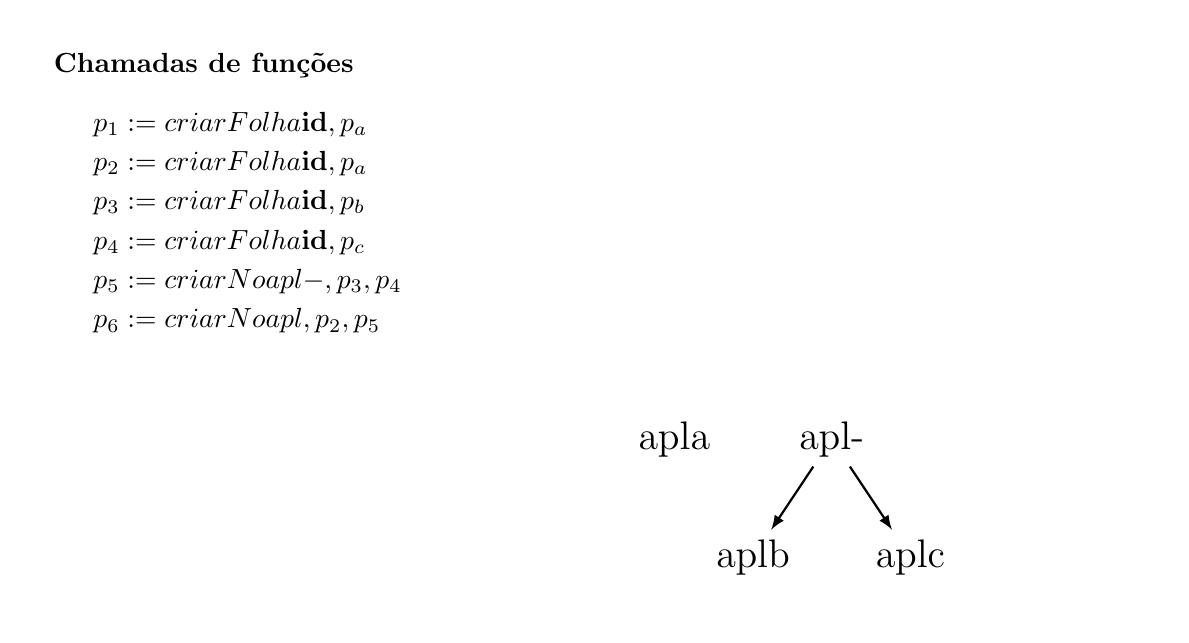
\begin{tikzpicture}
        \node[opacity=0] at (0, 0) { y };
        \node[opacity=0] at (14, 7) { t };

        \node[anchor=west] at (0, 6.75) { \textbf{Chamadas de funções} };
        \node[anchor=west] at (0.5, 6.0) { $p_1 := \Call{criarFolha}{\textbf{id}, p_a}$ };
        \node[anchor=west] at (0.5, 5.5) { $p_2 := \Call{criarFolha}{\textbf{id}, p_a}$ };
        \node[anchor=west] at (0.5, 5.0) { $p_3 := \Call{criarFolha}{\textbf{id}, p_b}$ };
        \node[anchor=west] at (0.5, 4.5) { $p_4 := \Call{criarFolha}{\textbf{id}, p_c}$ };
        \node[anchor=west] at (0.5, 4.0) { $p_5 := \Call{criarNo}{\code{apl}{-}, p_3, p_4}$ };
        \node[anchor=west] at (0.5, 3.5) { $p_6 := \Call{criarNo}{\code{apl}{×}, p_2, p_5}$ };
%        \node[anchor=west] at (0.5, 3.0) { $p_7 := \Call{criarFolha}{\textbf{id}, p_a}$ };
%        \node[anchor=west] at (0.5, 2.5) { $p_8 := \Call{criarFolha}{\textbf{id}, p_a}$ };
%        \node[anchor=west] at (0.5, 2.0) { $p_9 := \Call{criarFolha}{\textbf{id}, p_a}$ };
%        \node[anchor=west] at (0.5, 1.5) { $p_10 := \Call{criarFolha}{\textbf{id}, p_a}$ };
%        \node[anchor=west] at (0.5, 1.0) { $p_11 := \Call{criarFolha}{\textbf{id}, p_a}$ };
%        \node[anchor=west] at (0.5, 0.5) { $p_12 := \Call{criarFolha}{\textbf{id}, p_a}$ };
%        \node[anchor=west] at (0.5, 0.0) { $p_13 := \Call{criarFolha}{\textbf{id}, p_a}$ };

        \node (A) at (8, 2) { \Large \code{apl}{a} };
        \node (B) at (9, 0.5) { \Large \code{apl}{b} };
        \node (C) at (11, 0.5) { \Large \code{apl}{c} };
        \node (M) at (10, 2) { \Large \code{apl}{-} };

        \draw[thick,-latex] (M) to (B);
        \draw[thick,-latex] (M) to (C);

    \end{tikzpicture}

\end{frame}

\begin{frame}[fragile]{Criação do DAG para a expressão \code{apl}{a + a × (b - c) + (b - c) × d}}

    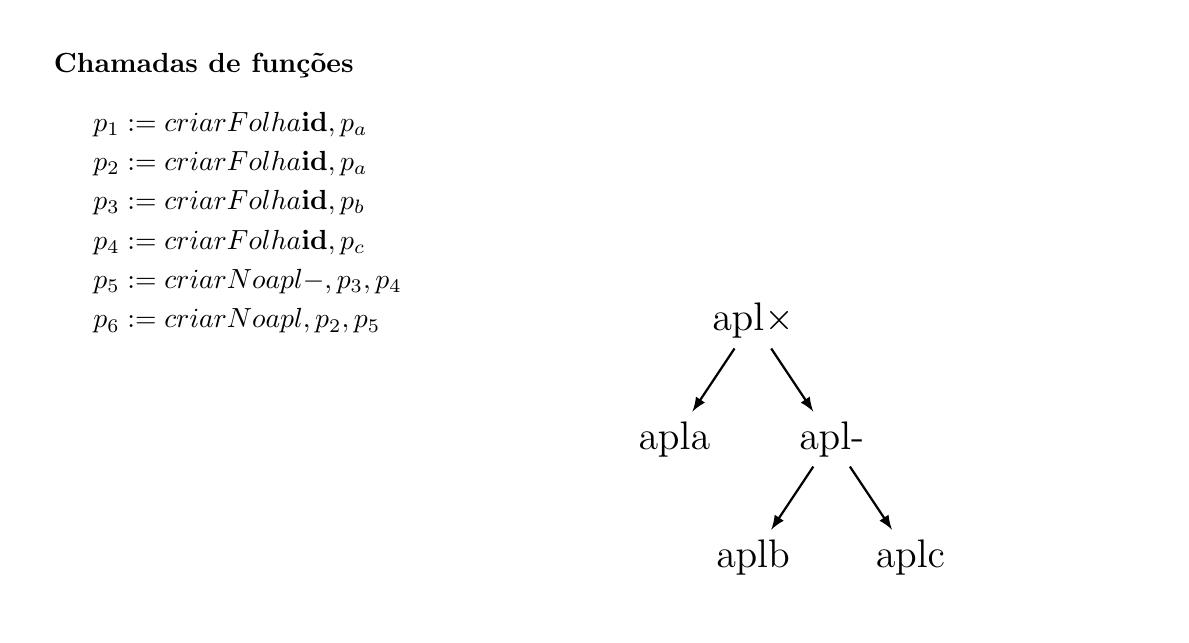
\begin{tikzpicture}
        \node[opacity=0] at (0, 0) { y };
        \node[opacity=0] at (14, 7) { t };

        \node[anchor=west] at (0, 6.75) { \textbf{Chamadas de funções} };
        \node[anchor=west] at (0.5, 6.0) { $p_1 := \Call{criarFolha}{\textbf{id}, p_a}$ };
        \node[anchor=west] at (0.5, 5.5) { $p_2 := \Call{criarFolha}{\textbf{id}, p_a}$ };
        \node[anchor=west] at (0.5, 5.0) { $p_3 := \Call{criarFolha}{\textbf{id}, p_b}$ };
        \node[anchor=west] at (0.5, 4.5) { $p_4 := \Call{criarFolha}{\textbf{id}, p_c}$ };
        \node[anchor=west] at (0.5, 4.0) { $p_5 := \Call{criarNo}{\code{apl}{-}, p_3, p_4}$ };
        \node[anchor=west] at (0.5, 3.5) { $p_6 := \Call{criarNo}{\code{apl}{×}, p_2, p_5}$ };
%        \node[anchor=west] at (0.5, 3.0) { $p_7 := \Call{criarFolha}{\textbf{id}, p_a}$ };
%        \node[anchor=west] at (0.5, 2.5) { $p_8 := \Call{criarFolha}{\textbf{id}, p_a}$ };
%        \node[anchor=west] at (0.5, 2.0) { $p_9 := \Call{criarFolha}{\textbf{id}, p_a}$ };
%        \node[anchor=west] at (0.5, 1.5) { $p_10 := \Call{criarFolha}{\textbf{id}, p_a}$ };
%        \node[anchor=west] at (0.5, 1.0) { $p_11 := \Call{criarFolha}{\textbf{id}, p_a}$ };
%        \node[anchor=west] at (0.5, 0.5) { $p_12 := \Call{criarFolha}{\textbf{id}, p_a}$ };
%        \node[anchor=west] at (0.5, 0.0) { $p_13 := \Call{criarFolha}{\textbf{id}, p_a}$ };

        \node (A) at (8, 2) { \Large \code{apl}{a} };
        \node (B) at (9, 0.5) { \Large \code{apl}{b} };
        \node (C) at (11, 0.5) { \Large \code{apl}{c} };
        \node (M) at (10, 2) { \Large \code{apl}{-} };
        \node (T1) at (9, 3.5) { \Large \code{apl}{×} };

        \draw[thick,-latex] (M) to (B);
        \draw[thick,-latex] (M) to (C);
        \draw[thick,-latex] (T1) to (M);
        \draw[thick,-latex] (T1) to (A);

    \end{tikzpicture}

\end{frame}

\begin{frame}[fragile]{Criação do DAG para a expressão \code{apl}{a + a × (b - c) + (b - c) × d}}

    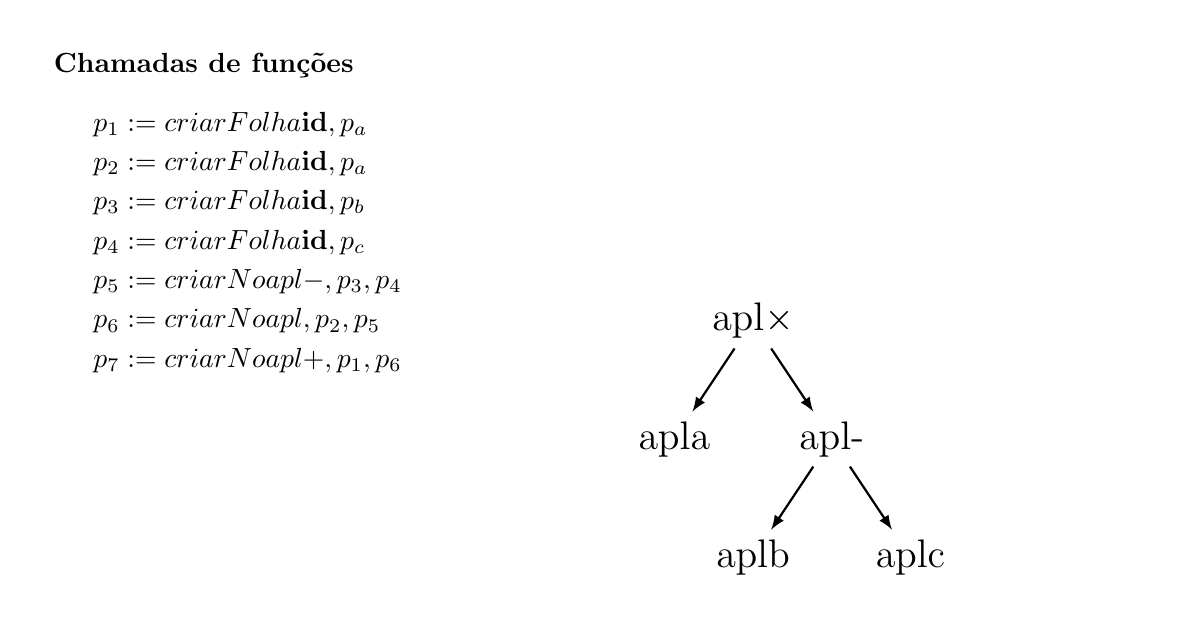
\begin{tikzpicture}
        \node[opacity=0] at (0, 0) { y };
        \node[opacity=0] at (14, 7) { t };

        \node[anchor=west] at (0, 6.75) { \textbf{Chamadas de funções} };
        \node[anchor=west] at (0.5, 6.0) { $p_1 := \Call{criarFolha}{\textbf{id}, p_a}$ };
        \node[anchor=west] at (0.5, 5.5) { $p_2 := \Call{criarFolha}{\textbf{id}, p_a}$ };
        \node[anchor=west] at (0.5, 5.0) { $p_3 := \Call{criarFolha}{\textbf{id}, p_b}$ };
        \node[anchor=west] at (0.5, 4.5) { $p_4 := \Call{criarFolha}{\textbf{id}, p_c}$ };
        \node[anchor=west] at (0.5, 4.0) { $p_5 := \Call{criarNo}{\code{apl}{-}, p_3, p_4}$ };
        \node[anchor=west] at (0.5, 3.5) { $p_6 := \Call{criarNo}{\code{apl}{×}, p_2, p_5}$ };
        \node[anchor=west] at (0.5, 3.0) { $p_7 := \Call{criarNo}{\code{apl}{+}, p_1, p_6}$ };
%        \node[anchor=west] at (0.5, 2.5) { $p_8 := \Call{criarFolha}{\textbf{id}, p_a}$ };
%        \node[anchor=west] at (0.5, 2.0) { $p_9 := \Call{criarFolha}{\textbf{id}, p_a}$ };
%        \node[anchor=west] at (0.5, 1.5) { $p_10 := \Call{criarFolha}{\textbf{id}, p_a}$ };
%        \node[anchor=west] at (0.5, 1.0) { $p_11 := \Call{criarFolha}{\textbf{id}, p_a}$ };
%        \node[anchor=west] at (0.5, 0.5) { $p_12 := \Call{criarFolha}{\textbf{id}, p_a}$ };
%        \node[anchor=west] at (0.5, 0.0) { $p_13 := \Call{criarFolha}{\textbf{id}, p_a}$ };

        \node (A) at (8, 2) { \Large \code{apl}{a} };
        \node (B) at (9, 0.5) { \Large \code{apl}{b} };
        \node (C) at (11, 0.5) { \Large \code{apl}{c} };
        \node (M) at (10, 2) { \Large \code{apl}{-} };
        \node (T1) at (9, 3.5) { \Large \code{apl}{×} };

        \draw[thick,-latex] (M) to (B);
        \draw[thick,-latex] (M) to (C);
        \draw[thick,-latex] (T1) to (M);
        \draw[thick,-latex] (T1) to (A);

    \end{tikzpicture}

\end{frame}

\begin{frame}[fragile]{Criação do DAG para a expressão \code{apl}{a + a × (b - c) + (b - c) × d}}

    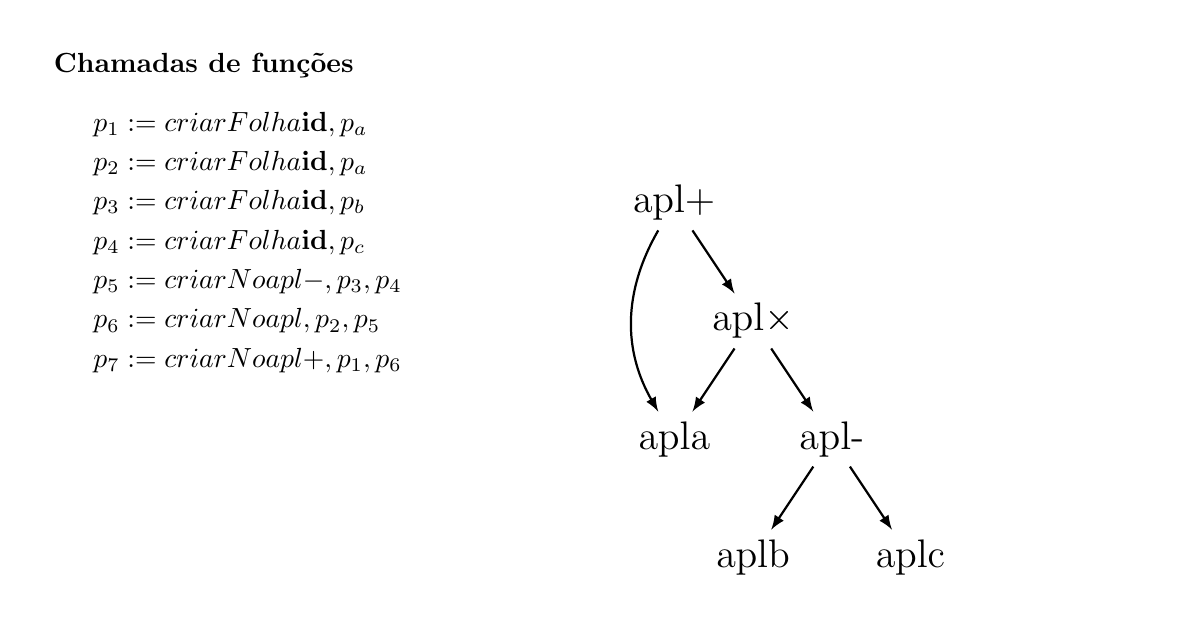
\begin{tikzpicture}
        \node[opacity=0] at (0, 0) { y };
        \node[opacity=0] at (14, 7) { t };

        \node[anchor=west] at (0, 6.75) { \textbf{Chamadas de funções} };
        \node[anchor=west] at (0.5, 6.0) { $p_1 := \Call{criarFolha}{\textbf{id}, p_a}$ };
        \node[anchor=west] at (0.5, 5.5) { $p_2 := \Call{criarFolha}{\textbf{id}, p_a}$ };
        \node[anchor=west] at (0.5, 5.0) { $p_3 := \Call{criarFolha}{\textbf{id}, p_b}$ };
        \node[anchor=west] at (0.5, 4.5) { $p_4 := \Call{criarFolha}{\textbf{id}, p_c}$ };
        \node[anchor=west] at (0.5, 4.0) { $p_5 := \Call{criarNo}{\code{apl}{-}, p_3, p_4}$ };
        \node[anchor=west] at (0.5, 3.5) { $p_6 := \Call{criarNo}{\code{apl}{×}, p_2, p_5}$ };
        \node[anchor=west] at (0.5, 3.0) { $p_7 := \Call{criarNo}{\code{apl}{+}, p_1, p_6}$ };
%        \node[anchor=west] at (0.5, 2.5) { $p_8 := \Call{criarFolha}{\textbf{id}, p_a}$ };
%        \node[anchor=west] at (0.5, 2.0) { $p_9 := \Call{criarFolha}{\textbf{id}, p_a}$ };
%        \node[anchor=west] at (0.5, 1.5) { $p_10 := \Call{criarFolha}{\textbf{id}, p_a}$ };
%        \node[anchor=west] at (0.5, 1.0) { $p_11 := \Call{criarFolha}{\textbf{id}, p_a}$ };
%        \node[anchor=west] at (0.5, 0.5) { $p_12 := \Call{criarFolha}{\textbf{id}, p_a}$ };
%        \node[anchor=west] at (0.5, 0.0) { $p_13 := \Call{criarFolha}{\textbf{id}, p_a}$ };

        \node (A) at (8, 2) { \Large \code{apl}{a} };
        \node (B) at (9, 0.5) { \Large \code{apl}{b} };
        \node (C) at (11, 0.5) { \Large \code{apl}{c} };
        \node (M) at (10, 2) { \Large \code{apl}{-} };
        \node (T1) at (9, 3.5) { \Large \code{apl}{×} };
        \node (P1) at (8, 5) { \Large \code{apl}{+} };

        \draw[thick,-latex] (M) to (B);
        \draw[thick,-latex] (M) to (C);
        \draw[thick,-latex] (T1) to (M);
        \draw[thick,-latex] (T1) to (A);
        \draw[thick,-latex] (P1) to [bend right] (A);
        \draw[thick,-latex] (P1) to (T1);

    \end{tikzpicture}

\end{frame}

\begin{frame}[fragile]{Criação do DAG para a expressão \code{apl}{a + a × (b - c) + (b - c) × d}}

    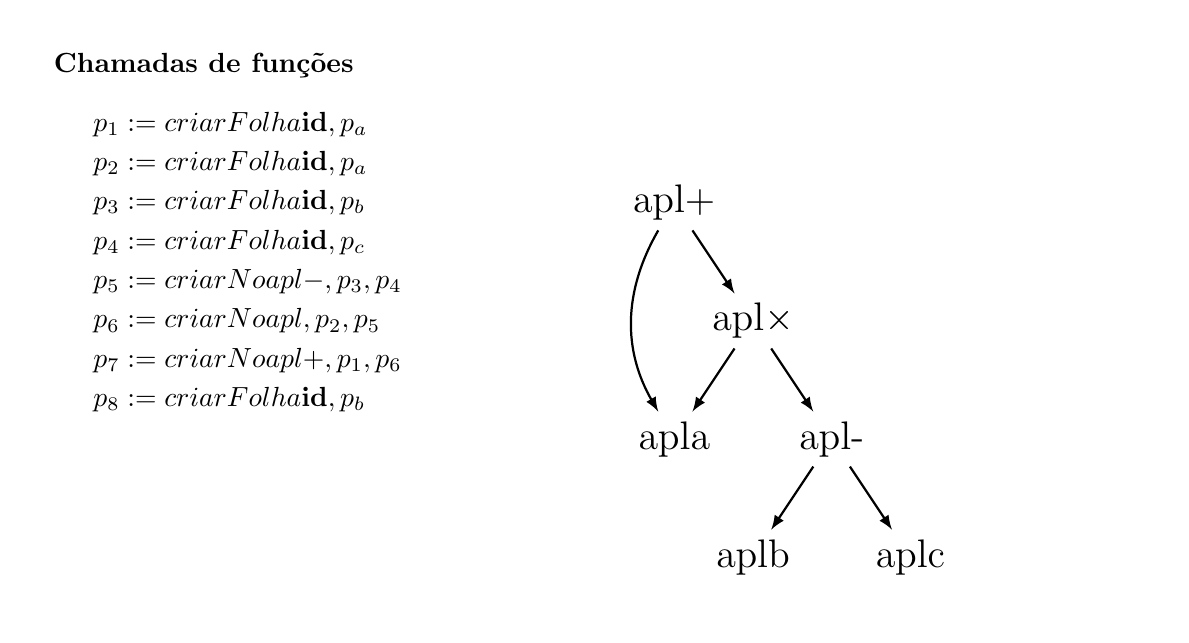
\begin{tikzpicture}
        \node[opacity=0] at (0, 0) { y };
        \node[opacity=0] at (14, 7) { t };

        \node[anchor=west] at (0, 6.75) { \textbf{Chamadas de funções} };
        \node[anchor=west] at (0.5, 6.0) { $p_1 := \Call{criarFolha}{\textbf{id}, p_a}$ };
        \node[anchor=west] at (0.5, 5.5) { $p_2 := \Call{criarFolha}{\textbf{id}, p_a}$ };
        \node[anchor=west] at (0.5, 5.0) { $p_3 := \Call{criarFolha}{\textbf{id}, p_b}$ };
        \node[anchor=west] at (0.5, 4.5) { $p_4 := \Call{criarFolha}{\textbf{id}, p_c}$ };
        \node[anchor=west] at (0.5, 4.0) { $p_5 := \Call{criarNo}{\code{apl}{-}, p_3, p_4}$ };
        \node[anchor=west] at (0.5, 3.5) { $p_6 := \Call{criarNo}{\code{apl}{×}, p_2, p_5}$ };
        \node[anchor=west] at (0.5, 3.0) { $p_7 := \Call{criarNo}{\code{apl}{+}, p_1, p_6}$ };
        \node[anchor=west] at (0.5, 2.5) { $p_8 := \Call{criarFolha}{\textbf{id}, p_b}$ };
%        \node[anchor=west] at (0.5, 2.0) { $p_9 := \Call{criarFolha}{\textbf{id}, p_a}$ };
%        \node[anchor=west] at (0.5, 1.5) { $p_10 := \Call{criarFolha}{\textbf{id}, p_a}$ };
%        \node[anchor=west] at (0.5, 1.0) { $p_11 := \Call{criarFolha}{\textbf{id}, p_a}$ };
%        \node[anchor=west] at (0.5, 0.5) { $p_12 := \Call{criarFolha}{\textbf{id}, p_a}$ };
%        \node[anchor=west] at (0.5, 0.0) { $p_13 := \Call{criarFolha}{\textbf{id}, p_a}$ };

        \node (A) at (8, 2) { \Large \code{apl}{a} };
        \node (B) at (9, 0.5) { \Large \code{apl}{b} };
        \node (C) at (11, 0.5) { \Large \code{apl}{c} };
        \node (M) at (10, 2) { \Large \code{apl}{-} };
        \node (T1) at (9, 3.5) { \Large \code{apl}{×} };
        \node (P1) at (8, 5) { \Large \code{apl}{+} };

        \draw[thick,-latex] (M) to (B);
        \draw[thick,-latex] (M) to (C);
        \draw[thick,-latex] (T1) to (M);
        \draw[thick,-latex] (T1) to (A);
        \draw[thick,-latex] (P1) to [bend right] (A);
        \draw[thick,-latex] (P1) to (T1);

    \end{tikzpicture}

\end{frame}

\begin{frame}[fragile]{Criação do DAG para a expressão \code{apl}{a + a × (b - c) + (b - c) × d}}

    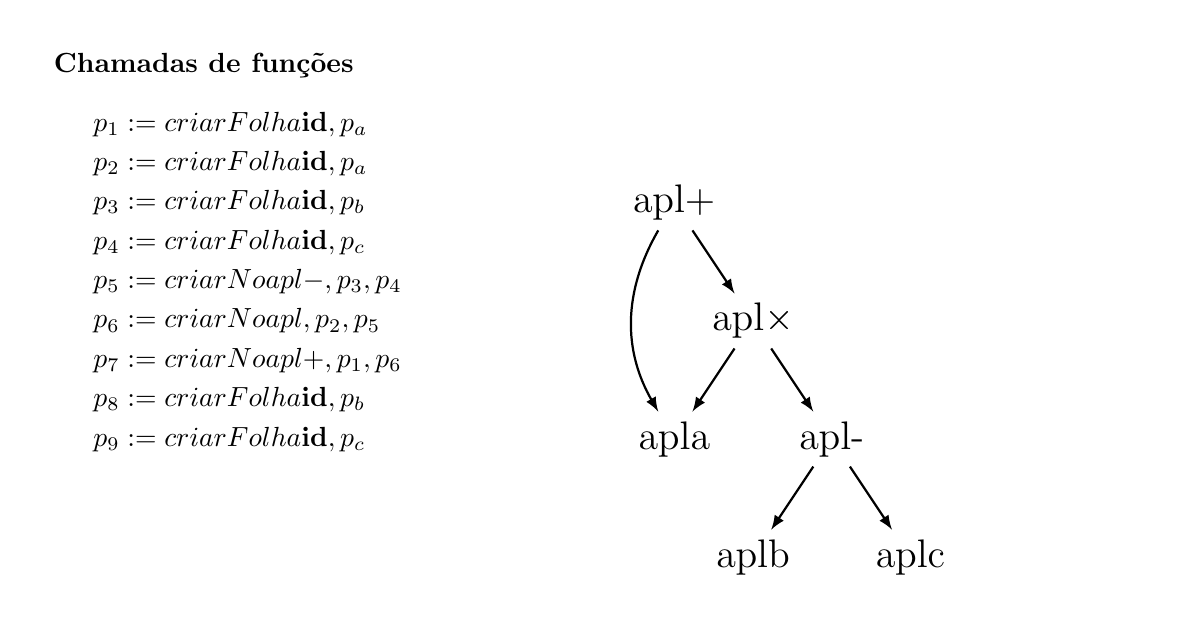
\begin{tikzpicture}
        \node[opacity=0] at (0, 0) { y };
        \node[opacity=0] at (14, 7) { t };

        \node[anchor=west] at (0, 6.75) { \textbf{Chamadas de funções} };
        \node[anchor=west] at (0.5, 6.0) { $p_1 := \Call{criarFolha}{\textbf{id}, p_a}$ };
        \node[anchor=west] at (0.5, 5.5) { $p_2 := \Call{criarFolha}{\textbf{id}, p_a}$ };
        \node[anchor=west] at (0.5, 5.0) { $p_3 := \Call{criarFolha}{\textbf{id}, p_b}$ };
        \node[anchor=west] at (0.5, 4.5) { $p_4 := \Call{criarFolha}{\textbf{id}, p_c}$ };
        \node[anchor=west] at (0.5, 4.0) { $p_5 := \Call{criarNo}{\code{apl}{-}, p_3, p_4}$ };
        \node[anchor=west] at (0.5, 3.5) { $p_6 := \Call{criarNo}{\code{apl}{×}, p_2, p_5}$ };
        \node[anchor=west] at (0.5, 3.0) { $p_7 := \Call{criarNo}{\code{apl}{+}, p_1, p_6}$ };
        \node[anchor=west] at (0.5, 2.5) { $p_8 := \Call{criarFolha}{\textbf{id}, p_b}$ };
        \node[anchor=west] at (0.5, 2.0) { $p_9 := \Call{criarFolha}{\textbf{id}, p_c}$ };
%        \node[anchor=west] at (0.5, 1.5) { $p_10 := \Call{criarFolha}{\textbf{id}, p_a}$ };
%        \node[anchor=west] at (0.5, 1.0) { $p_11 := \Call{criarFolha}{\textbf{id}, p_a}$ };
%        \node[anchor=west] at (0.5, 0.5) { $p_12 := \Call{criarFolha}{\textbf{id}, p_a}$ };
%        \node[anchor=west] at (0.5, 0.0) { $p_13 := \Call{criarFolha}{\textbf{id}, p_a}$ };

        \node (A) at (8, 2) { \Large \code{apl}{a} };
        \node (B) at (9, 0.5) { \Large \code{apl}{b} };
        \node (C) at (11, 0.5) { \Large \code{apl}{c} };
        \node (M) at (10, 2) { \Large \code{apl}{-} };
        \node (T1) at (9, 3.5) { \Large \code{apl}{×} };
        \node (P1) at (8, 5) { \Large \code{apl}{+} };

        \draw[thick,-latex] (M) to (B);
        \draw[thick,-latex] (M) to (C);
        \draw[thick,-latex] (T1) to (M);
        \draw[thick,-latex] (T1) to (A);
        \draw[thick,-latex] (P1) to [bend right] (A);
        \draw[thick,-latex] (P1) to (T1);

    \end{tikzpicture}

\end{frame}

\begin{frame}[fragile]{Criação do DAG para a expressão \code{apl}{a + a × (b - c) + (b - c) × d}}

    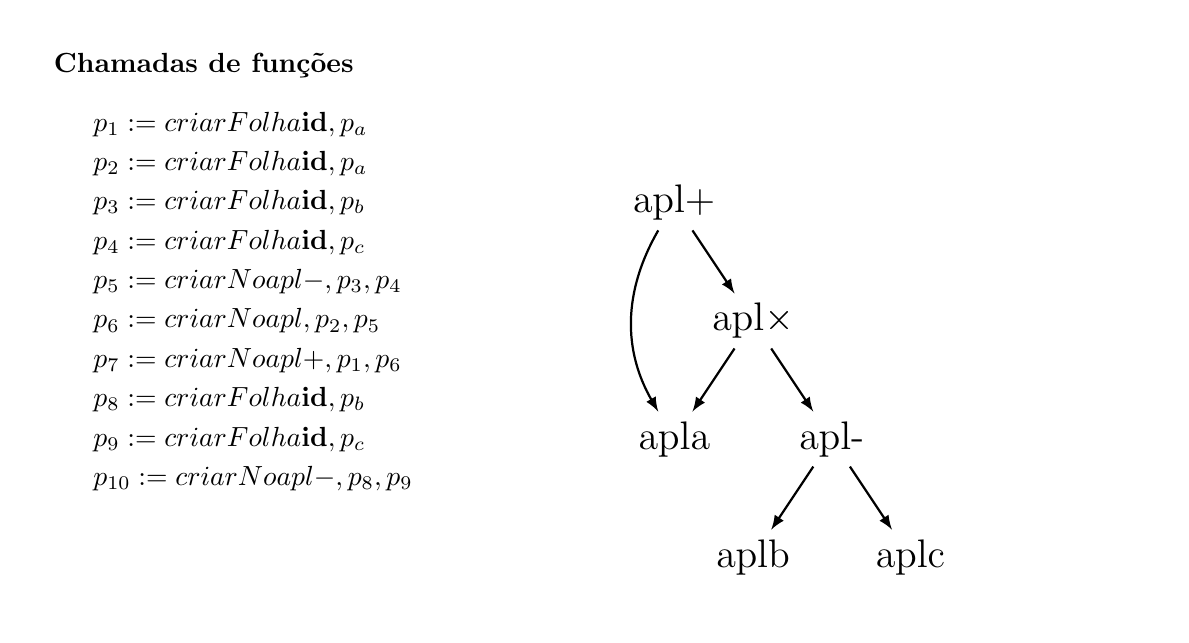
\begin{tikzpicture}
        \node[opacity=0] at (0, 0) { y };
        \node[opacity=0] at (14, 7) { t };

        \node[anchor=west] at (0, 6.75) { \textbf{Chamadas de funções} };
        \node[anchor=west] at (0.5, 6.0) { $p_1 := \Call{criarFolha}{\textbf{id}, p_a}$ };
        \node[anchor=west] at (0.5, 5.5) { $p_2 := \Call{criarFolha}{\textbf{id}, p_a}$ };
        \node[anchor=west] at (0.5, 5.0) { $p_3 := \Call{criarFolha}{\textbf{id}, p_b}$ };
        \node[anchor=west] at (0.5, 4.5) { $p_4 := \Call{criarFolha}{\textbf{id}, p_c}$ };
        \node[anchor=west] at (0.5, 4.0) { $p_5 := \Call{criarNo}{\code{apl}{-}, p_3, p_4}$ };
        \node[anchor=west] at (0.5, 3.5) { $p_6 := \Call{criarNo}{\code{apl}{×}, p_2, p_5}$ };
        \node[anchor=west] at (0.5, 3.0) { $p_7 := \Call{criarNo}{\code{apl}{+}, p_1, p_6}$ };
        \node[anchor=west] at (0.5, 2.5) { $p_8 := \Call{criarFolha}{\textbf{id}, p_b}$ };
        \node[anchor=west] at (0.5, 2.0) { $p_9 := \Call{criarFolha}{\textbf{id}, p_c}$ };
        \node[anchor=west] at (0.5, 1.5) { $p_{10} := \Call{criarNo}{\code{apl}{-}, p_8, p_9}$ };
%        \node[anchor=west] at (0.5, 1.0) { $p_11 := \Call{criarFolha}{\textbf{id}, p_a}$ };
%        \node[anchor=west] at (0.5, 0.5) { $p_12 := \Call{criarFolha}{\textbf{id}, p_a}$ };
%        \node[anchor=west] at (0.5, 0.0) { $p_13 := \Call{criarFolha}{\textbf{id}, p_a}$ };

        \node (A) at (8, 2) { \Large \code{apl}{a} };
        \node (B) at (9, 0.5) { \Large \code{apl}{b} };
        \node (C) at (11, 0.5) { \Large \code{apl}{c} };
        \node (M) at (10, 2) { \Large \code{apl}{-} };
        \node (T1) at (9, 3.5) { \Large \code{apl}{×} };
        \node (P1) at (8, 5) { \Large \code{apl}{+} };

        \draw[thick,-latex] (M) to (B);
        \draw[thick,-latex] (M) to (C);
        \draw[thick,-latex] (T1) to (M);
        \draw[thick,-latex] (T1) to (A);
        \draw[thick,-latex] (P1) to [bend right] (A);
        \draw[thick,-latex] (P1) to (T1);

    \end{tikzpicture}

\end{frame}

\begin{frame}[fragile]{Criação do DAG para a expressão \code{apl}{a + a × (b - c) + (b - c) × d}}

    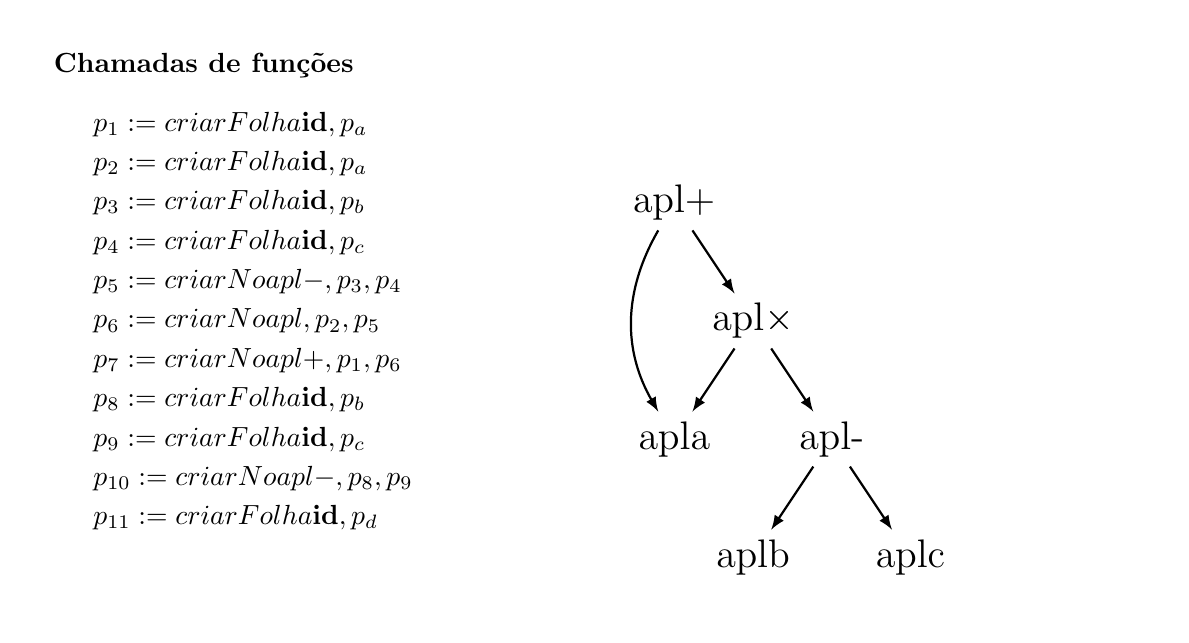
\begin{tikzpicture}
        \node[opacity=0] at (0, 0) { y };
        \node[opacity=0] at (14, 7) { t };

        \node[anchor=west] at (0, 6.75) { \textbf{Chamadas de funções} };
        \node[anchor=west] at (0.5, 6.0) { $p_1 := \Call{criarFolha}{\textbf{id}, p_a}$ };
        \node[anchor=west] at (0.5, 5.5) { $p_2 := \Call{criarFolha}{\textbf{id}, p_a}$ };
        \node[anchor=west] at (0.5, 5.0) { $p_3 := \Call{criarFolha}{\textbf{id}, p_b}$ };
        \node[anchor=west] at (0.5, 4.5) { $p_4 := \Call{criarFolha}{\textbf{id}, p_c}$ };
        \node[anchor=west] at (0.5, 4.0) { $p_5 := \Call{criarNo}{\code{apl}{-}, p_3, p_4}$ };
        \node[anchor=west] at (0.5, 3.5) { $p_6 := \Call{criarNo}{\code{apl}{×}, p_2, p_5}$ };
        \node[anchor=west] at (0.5, 3.0) { $p_7 := \Call{criarNo}{\code{apl}{+}, p_1, p_6}$ };
        \node[anchor=west] at (0.5, 2.5) { $p_8 := \Call{criarFolha}{\textbf{id}, p_b}$ };
        \node[anchor=west] at (0.5, 2.0) { $p_9 := \Call{criarFolha}{\textbf{id}, p_c}$ };
        \node[anchor=west] at (0.5, 1.5) { $p_{10} := \Call{criarNo}{\code{apl}{-}, p_8, p_9}$ };
        \node[anchor=west] at (0.5, 1.0) { $p_{11} := \Call{criarFolha}{\textbf{id}, p_d}$ };
%        \node[anchor=west] at (0.5, 0.5) { $p_12 := \Call{criarFolha}{\textbf{id}, p_a}$ };
%        \node[anchor=west] at (0.5, 0.0) { $p_13 := \Call{criarFolha}{\textbf{id}, p_a}$ };

        \node (A) at (8, 2) { \Large \code{apl}{a} };
        \node (B) at (9, 0.5) { \Large \code{apl}{b} };
        \node (C) at (11, 0.5) { \Large \code{apl}{c} };
        \node (M) at (10, 2) { \Large \code{apl}{-} };
        \node (T1) at (9, 3.5) { \Large \code{apl}{×} };
        \node (P1) at (8, 5) { \Large \code{apl}{+} };

        \draw[thick,-latex] (M) to (B);
        \draw[thick,-latex] (M) to (C);
        \draw[thick,-latex] (T1) to (M);
        \draw[thick,-latex] (T1) to (A);
        \draw[thick,-latex] (P1) to [bend right] (A);
        \draw[thick,-latex] (P1) to (T1);

    \end{tikzpicture}

\end{frame}

\begin{frame}[fragile]{Criação do DAG para a expressão \code{apl}{a + a × (b - c) + (b - c) × d}}

    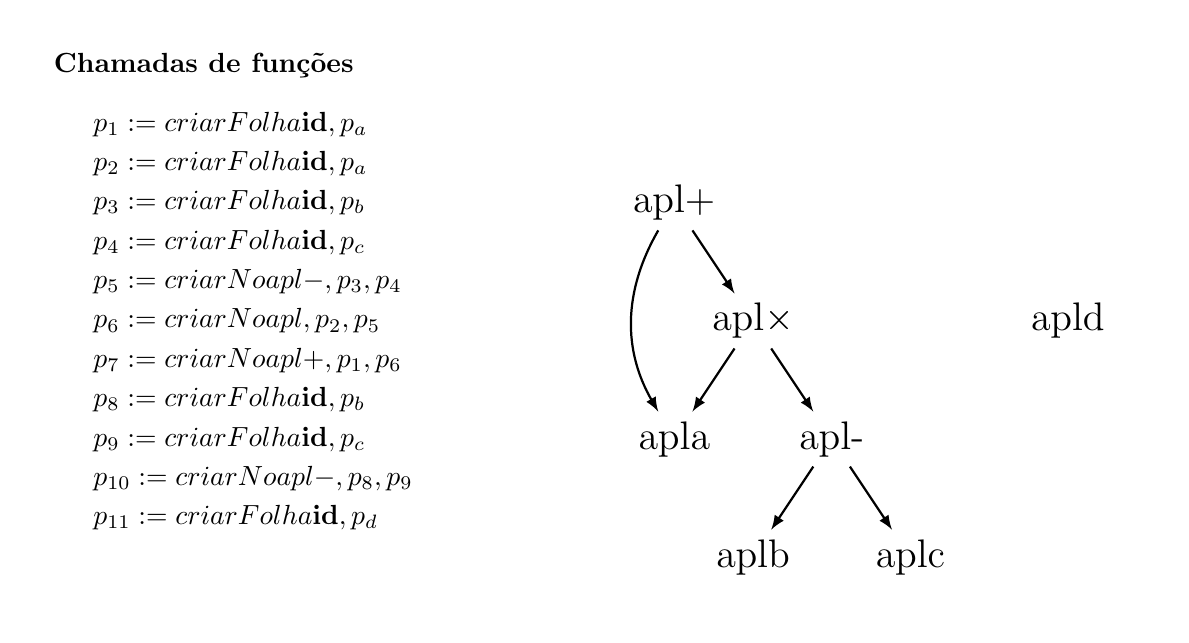
\begin{tikzpicture}
        \node[opacity=0] at (0, 0) { y };
        \node[opacity=0] at (14, 7) { t };

        \node[anchor=west] at (0, 6.75) { \textbf{Chamadas de funções} };
        \node[anchor=west] at (0.5, 6.0) { $p_1 := \Call{criarFolha}{\textbf{id}, p_a}$ };
        \node[anchor=west] at (0.5, 5.5) { $p_2 := \Call{criarFolha}{\textbf{id}, p_a}$ };
        \node[anchor=west] at (0.5, 5.0) { $p_3 := \Call{criarFolha}{\textbf{id}, p_b}$ };
        \node[anchor=west] at (0.5, 4.5) { $p_4 := \Call{criarFolha}{\textbf{id}, p_c}$ };
        \node[anchor=west] at (0.5, 4.0) { $p_5 := \Call{criarNo}{\code{apl}{-}, p_3, p_4}$ };
        \node[anchor=west] at (0.5, 3.5) { $p_6 := \Call{criarNo}{\code{apl}{×}, p_2, p_5}$ };
        \node[anchor=west] at (0.5, 3.0) { $p_7 := \Call{criarNo}{\code{apl}{+}, p_1, p_6}$ };
        \node[anchor=west] at (0.5, 2.5) { $p_8 := \Call{criarFolha}{\textbf{id}, p_b}$ };
        \node[anchor=west] at (0.5, 2.0) { $p_9 := \Call{criarFolha}{\textbf{id}, p_c}$ };
        \node[anchor=west] at (0.5, 1.5) { $p_{10} := \Call{criarNo}{\code{apl}{-}, p_8, p_9}$ };
        \node[anchor=west] at (0.5, 1.0) { $p_{11} := \Call{criarFolha}{\textbf{id}, p_d}$ };
%        \node[anchor=west] at (0.5, 0.5) { $p_12 := \Call{criarFolha}{\textbf{id}, p_a}$ };
%        \node[anchor=west] at (0.5, 0.0) { $p_13 := \Call{criarFolha}{\textbf{id}, p_a}$ };

        \node (A) at (8, 2) { \Large \code{apl}{a} };
        \node (B) at (9, 0.5) { \Large \code{apl}{b} };
        \node (C) at (11, 0.5) { \Large \code{apl}{c} };
        \node (M) at (10, 2) { \Large \code{apl}{-} };
        \node (T1) at (9, 3.5) { \Large \code{apl}{×} };
        \node (P1) at (8, 5) { \Large \code{apl}{+} };
        \node (D) at (13, 3.5) { \Large \code{apl}{d} };

        \draw[thick,-latex] (M) to (B);
        \draw[thick,-latex] (M) to (C);
        \draw[thick,-latex] (T1) to (M);
        \draw[thick,-latex] (T1) to (A);
        \draw[thick,-latex] (P1) to [bend right] (A);
        \draw[thick,-latex] (P1) to (T1);

    \end{tikzpicture}

\end{frame}

\begin{frame}[fragile]{Criação do DAG para a expressão \code{apl}{a + a × (b - c) + (b - c) × d}}

    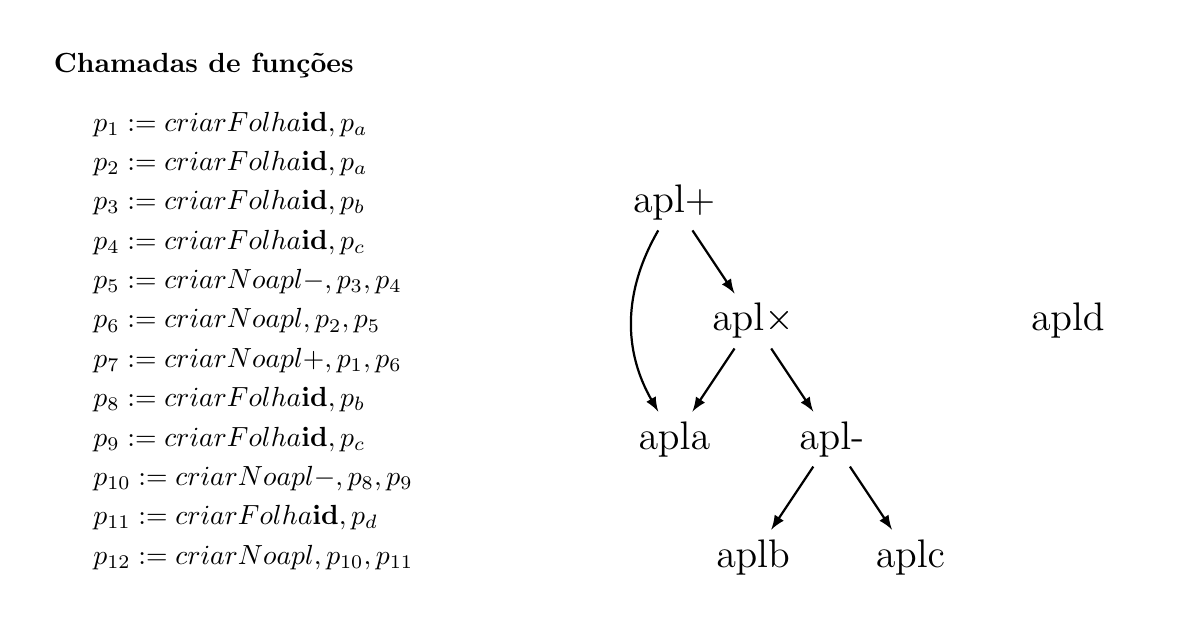
\begin{tikzpicture}
        \node[opacity=0] at (0, 0) { y };
        \node[opacity=0] at (14, 7) { t };

        \node[anchor=west] at (0, 6.75) { \textbf{Chamadas de funções} };
        \node[anchor=west] at (0.5, 6.0) { $p_1 := \Call{criarFolha}{\textbf{id}, p_a}$ };
        \node[anchor=west] at (0.5, 5.5) { $p_2 := \Call{criarFolha}{\textbf{id}, p_a}$ };
        \node[anchor=west] at (0.5, 5.0) { $p_3 := \Call{criarFolha}{\textbf{id}, p_b}$ };
        \node[anchor=west] at (0.5, 4.5) { $p_4 := \Call{criarFolha}{\textbf{id}, p_c}$ };
        \node[anchor=west] at (0.5, 4.0) { $p_5 := \Call{criarNo}{\code{apl}{-}, p_3, p_4}$ };
        \node[anchor=west] at (0.5, 3.5) { $p_6 := \Call{criarNo}{\code{apl}{×}, p_2, p_5}$ };
        \node[anchor=west] at (0.5, 3.0) { $p_7 := \Call{criarNo}{\code{apl}{+}, p_1, p_6}$ };
        \node[anchor=west] at (0.5, 2.5) { $p_8 := \Call{criarFolha}{\textbf{id}, p_b}$ };
        \node[anchor=west] at (0.5, 2.0) { $p_9 := \Call{criarFolha}{\textbf{id}, p_c}$ };
        \node[anchor=west] at (0.5, 1.5) { $p_{10} := \Call{criarNo}{\code{apl}{-}, p_8, p_9}$ };
        \node[anchor=west] at (0.5, 1.0) { $p_{11} := \Call{criarFolha}{\textbf{id}, p_d}$ };
        \node[anchor=west] at (0.5, 0.5) { $p_{12} := \Call{criarNo}{\code{apl}{×}, p_{10}, p_{11}}$ };
%        \node[anchor=west] at (0.5, 0.0) { $p_13 := \Call{criarFolha}{\textbf{id}, p_a}$ };

        \node (A) at (8, 2) { \Large \code{apl}{a} };
        \node (B) at (9, 0.5) { \Large \code{apl}{b} };
        \node (C) at (11, 0.5) { \Large \code{apl}{c} };
        \node (M) at (10, 2) { \Large \code{apl}{-} };
        \node (T1) at (9, 3.5) { \Large \code{apl}{×} };
        \node (P1) at (8, 5) { \Large \code{apl}{+} };
        \node (D) at (13, 3.5) { \Large \code{apl}{d} };

        \draw[thick,-latex] (M) to (B);
        \draw[thick,-latex] (M) to (C);
        \draw[thick,-latex] (T1) to (M);
        \draw[thick,-latex] (T1) to (A);
        \draw[thick,-latex] (P1) to [bend right] (A);
        \draw[thick,-latex] (P1) to (T1);

    \end{tikzpicture}

\end{frame}

\begin{frame}[fragile]{Criação do DAG para a expressão \code{apl}{a + a × (b - c) + (b - c) × d}}

    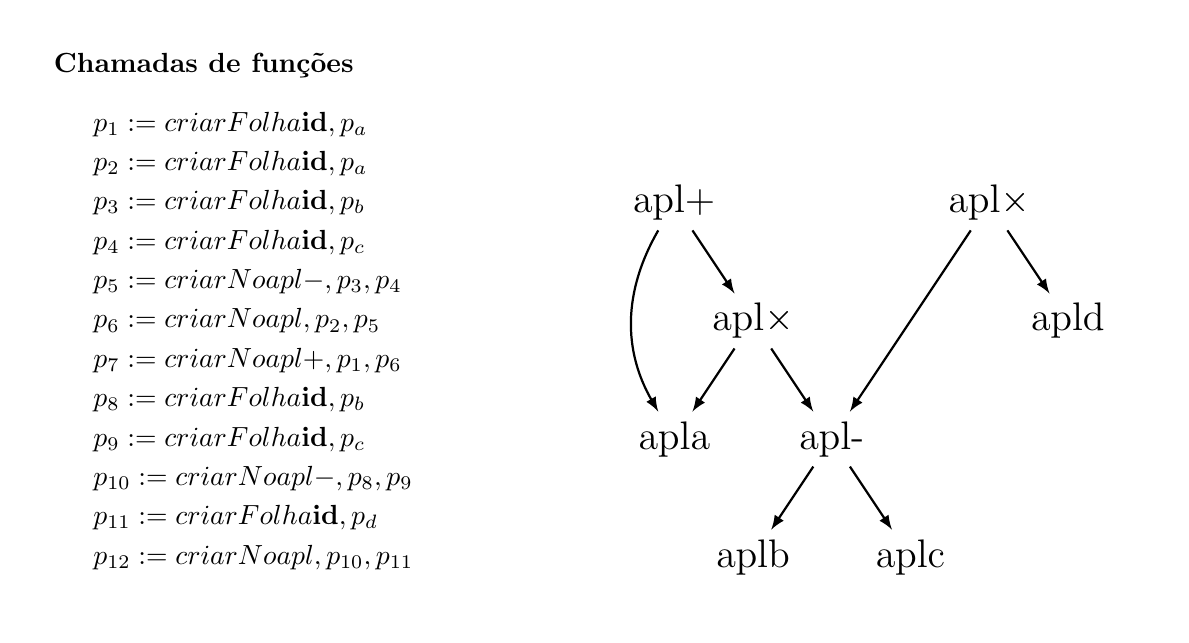
\begin{tikzpicture}
        \node[opacity=0] at (0, 0) { y };
        \node[opacity=0] at (14, 7) { t };

        \node[anchor=west] at (0, 6.75) { \textbf{Chamadas de funções} };
        \node[anchor=west] at (0.5, 6.0) { $p_1 := \Call{criarFolha}{\textbf{id}, p_a}$ };
        \node[anchor=west] at (0.5, 5.5) { $p_2 := \Call{criarFolha}{\textbf{id}, p_a}$ };
        \node[anchor=west] at (0.5, 5.0) { $p_3 := \Call{criarFolha}{\textbf{id}, p_b}$ };
        \node[anchor=west] at (0.5, 4.5) { $p_4 := \Call{criarFolha}{\textbf{id}, p_c}$ };
        \node[anchor=west] at (0.5, 4.0) { $p_5 := \Call{criarNo}{\code{apl}{-}, p_3, p_4}$ };
        \node[anchor=west] at (0.5, 3.5) { $p_6 := \Call{criarNo}{\code{apl}{×}, p_2, p_5}$ };
        \node[anchor=west] at (0.5, 3.0) { $p_7 := \Call{criarNo}{\code{apl}{+}, p_1, p_6}$ };
        \node[anchor=west] at (0.5, 2.5) { $p_8 := \Call{criarFolha}{\textbf{id}, p_b}$ };
        \node[anchor=west] at (0.5, 2.0) { $p_9 := \Call{criarFolha}{\textbf{id}, p_c}$ };
        \node[anchor=west] at (0.5, 1.5) { $p_{10} := \Call{criarNo}{\code{apl}{-}, p_8, p_9}$ };
        \node[anchor=west] at (0.5, 1.0) { $p_{11} := \Call{criarFolha}{\textbf{id}, p_d}$ };
        \node[anchor=west] at (0.5, 0.5) { $p_{12} := \Call{criarNo}{\code{apl}{×}, p_{10}, p_{11}}$ };
%        \node[anchor=west] at (0.5, 0.0) { $p_13 := \Call{criarFolha}{\textbf{id}, p_a}$ };

        \node (A) at (8, 2) { \Large \code{apl}{a} };
        \node (B) at (9, 0.5) { \Large \code{apl}{b} };
        \node (C) at (11, 0.5) { \Large \code{apl}{c} };
        \node (M) at (10, 2) { \Large \code{apl}{-} };
        \node (T1) at (9, 3.5) { \Large \code{apl}{×} };
        \node (P1) at (8, 5) { \Large \code{apl}{+} };
        \node (D) at (13, 3.5) { \Large \code{apl}{d} };
        \node (T2) at (12, 5) { \Large \code{apl}{×} };

        \draw[thick,-latex] (M) to (B);
        \draw[thick,-latex] (M) to (C);
        \draw[thick,-latex] (T1) to (M);
        \draw[thick,-latex] (T1) to (A);
        \draw[thick,-latex] (P1) to [bend right] (A);
        \draw[thick,-latex] (P1) to (T1);
        \draw[thick,-latex] (T2) to (D);
        \draw[thick,-latex] (T2) to (M);

    \end{tikzpicture}

\end{frame}

\begin{frame}[fragile]{Criação do DAG para a expressão \code{apl}{a + a × (b - c) + (b - c) × d}}

    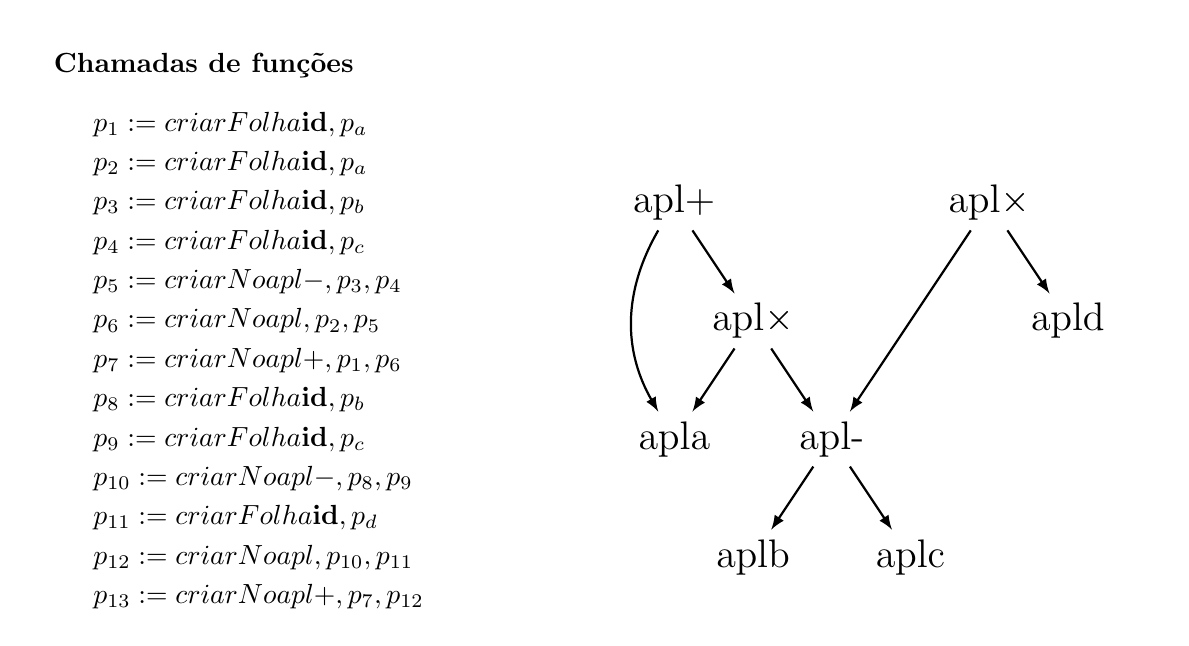
\begin{tikzpicture}
        \node[opacity=0] at (0, 0) { y };
        \node[opacity=0] at (14, 7) { t };

        \node[anchor=west] at (0, 6.75) { \textbf{Chamadas de funções} };
        \node[anchor=west] at (0.5, 6.0) { $p_1 := \Call{criarFolha}{\textbf{id}, p_a}$ };
        \node[anchor=west] at (0.5, 5.5) { $p_2 := \Call{criarFolha}{\textbf{id}, p_a}$ };
        \node[anchor=west] at (0.5, 5.0) { $p_3 := \Call{criarFolha}{\textbf{id}, p_b}$ };
        \node[anchor=west] at (0.5, 4.5) { $p_4 := \Call{criarFolha}{\textbf{id}, p_c}$ };
        \node[anchor=west] at (0.5, 4.0) { $p_5 := \Call{criarNo}{\code{apl}{-}, p_3, p_4}$ };
        \node[anchor=west] at (0.5, 3.5) { $p_6 := \Call{criarNo}{\code{apl}{×}, p_2, p_5}$ };
        \node[anchor=west] at (0.5, 3.0) { $p_7 := \Call{criarNo}{\code{apl}{+}, p_1, p_6}$ };
        \node[anchor=west] at (0.5, 2.5) { $p_8 := \Call{criarFolha}{\textbf{id}, p_b}$ };
        \node[anchor=west] at (0.5, 2.0) { $p_9 := \Call{criarFolha}{\textbf{id}, p_c}$ };
        \node[anchor=west] at (0.5, 1.5) { $p_{10} := \Call{criarNo}{\code{apl}{-}, p_8, p_9}$ };
        \node[anchor=west] at (0.5, 1.0) { $p_{11} := \Call{criarFolha}{\textbf{id}, p_d}$ };
        \node[anchor=west] at (0.5, 0.5) { $p_{12} := \Call{criarNo}{\code{apl}{×}, p_{10}, p_{11}}$ };
        \node[anchor=west] at (0.5, 0.0) { $p_{13} := \Call{criarNo}{\code{apl}{+}, p_{7}, p_{12}}$ };

        \node (A) at (8, 2) { \Large \code{apl}{a} };
        \node (B) at (9, 0.5) { \Large \code{apl}{b} };
        \node (C) at (11, 0.5) { \Large \code{apl}{c} };
        \node (M) at (10, 2) { \Large \code{apl}{-} };
        \node (T1) at (9, 3.5) { \Large \code{apl}{×} };
        \node (P1) at (8, 5) { \Large \code{apl}{+} };
        \node (D) at (13, 3.5) { \Large \code{apl}{d} };
        \node (T2) at (12, 5) { \Large \code{apl}{×} };

        \draw[thick,-latex] (M) to (B);
        \draw[thick,-latex] (M) to (C);
        \draw[thick,-latex] (T1) to (M);
        \draw[thick,-latex] (T1) to (A);
        \draw[thick,-latex] (P1) to [bend right] (A);
        \draw[thick,-latex] (P1) to (T1);
        \draw[thick,-latex] (T2) to (D);
        \draw[thick,-latex] (T2) to (M);

    \end{tikzpicture}

\end{frame}

\begin{frame}[fragile]{Criação do DAG para a expressão \code{apl}{a + a × (b - c) + (b - c) × d}}

    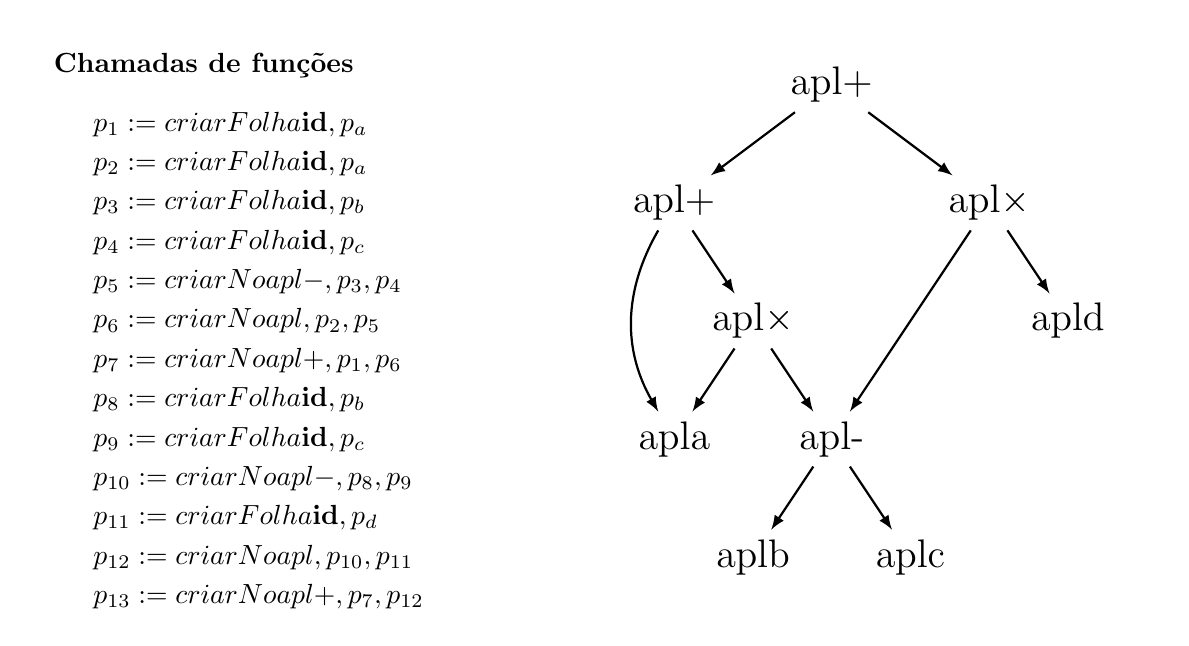
\begin{tikzpicture}
        \node[opacity=0] at (0, 0) { y };
        \node[opacity=0] at (14, 7) { t };

        \node[anchor=west] at (0, 6.75) { \textbf{Chamadas de funções} };
        \node[anchor=west] at (0.5, 6.0) { $p_1 := \Call{criarFolha}{\textbf{id}, p_a}$ };
        \node[anchor=west] at (0.5, 5.5) { $p_2 := \Call{criarFolha}{\textbf{id}, p_a}$ };
        \node[anchor=west] at (0.5, 5.0) { $p_3 := \Call{criarFolha}{\textbf{id}, p_b}$ };
        \node[anchor=west] at (0.5, 4.5) { $p_4 := \Call{criarFolha}{\textbf{id}, p_c}$ };
        \node[anchor=west] at (0.5, 4.0) { $p_5 := \Call{criarNo}{\code{apl}{-}, p_3, p_4}$ };
        \node[anchor=west] at (0.5, 3.5) { $p_6 := \Call{criarNo}{\code{apl}{×}, p_2, p_5}$ };
        \node[anchor=west] at (0.5, 3.0) { $p_7 := \Call{criarNo}{\code{apl}{+}, p_1, p_6}$ };
        \node[anchor=west] at (0.5, 2.5) { $p_8 := \Call{criarFolha}{\textbf{id}, p_b}$ };
        \node[anchor=west] at (0.5, 2.0) { $p_9 := \Call{criarFolha}{\textbf{id}, p_c}$ };
        \node[anchor=west] at (0.5, 1.5) { $p_{10} := \Call{criarNo}{\code{apl}{-}, p_8, p_9}$ };
        \node[anchor=west] at (0.5, 1.0) { $p_{11} := \Call{criarFolha}{\textbf{id}, p_d}$ };
        \node[anchor=west] at (0.5, 0.5) { $p_{12} := \Call{criarNo}{\code{apl}{×}, p_{10}, p_{11}}$ };
        \node[anchor=west] at (0.5, 0.0) { $p_{13} := \Call{criarNo}{\code{apl}{+}, p_{7}, p_{12}}$ };

        \node (A) at (8, 2) { \Large \code{apl}{a} };
        \node (B) at (9, 0.5) { \Large \code{apl}{b} };
        \node (C) at (11, 0.5) { \Large \code{apl}{c} };
        \node (M) at (10, 2) { \Large \code{apl}{-} };
        \node (T1) at (9, 3.5) { \Large \code{apl}{×} };
        \node (P1) at (8, 5) { \Large \code{apl}{+} };
        \node (D) at (13, 3.5) { \Large \code{apl}{d} };
        \node (T2) at (12, 5) { \Large \code{apl}{×} };
        \node (P2) at (10, 6.5) { \Large \code{apl}{+} };

        \draw[thick,-latex] (M) to (B);
        \draw[thick,-latex] (M) to (C);
        \draw[thick,-latex] (T1) to (M);
        \draw[thick,-latex] (T1) to (A);
        \draw[thick,-latex] (P1) to [bend right] (A);
        \draw[thick,-latex] (P1) to (T1);
        \draw[thick,-latex] (T2) to (D);
        \draw[thick,-latex] (T2) to (M);
        \draw[thick,-latex] (P2) to (P1);
        \draw[thick,-latex] (P2) to (T2);

    \end{tikzpicture}

\end{frame}
